\section{Examples}
\subsection{The octahedron}

We will define some higher inductive types to serve as domain and codomain of these motivating examples.

\subsubsection{The higher inductive type \( \oo \)}

First we need a square, which will be a stand-in for a circle that can support a notion of a quarter-rotation. 

\begin{mydef}
The higher inductive type \( C_4 \) (where C stands for ``circle'').
\begin{align*}
C_4 &: \Type \\
c_1, c_2, c_3, c_4 &: C_4 \\
c_1c_2 &: c_1 = c_2 \\
c_2c_3 &: c_2 = c_3 \\
c_3c_4 &: c_3 = c_4 \\
c_4c_1 &: c_4 = c_1 \\
\end{align*}
\end{mydef}

\begin{figure}[h]
\centering
\begin{tikzpicture}[
node distance = 15mm and 15mm,
V/.style = {circle, fill, draw=black, inner sep=1pt, font=\footnotesize},
every edge quotes/.style = {auto, font=\footnotesize},
arrow/.style={->,semithick}
]
\begin{scope}[nodes=V]
  \node[label=above left:\( c_1 \)] (1) {};
  \node[label=above right:\( c_2 \)] (2) [right=of 1]  {};
  \node[label=below right:\( c_3 \)] (3) [below=of 2]  {};
  \node[label=below left:\( c_4 \)] (4) [below=of 1]  {};
\end{scope}
\draw[arrow]
        (1)  edge["\( c_1c_2 \)"] (2)
        (2)  edge["\( c_2c_3 \)"] (3)
        (3)  edge["\( c_3c_4 \)"] (4)
        (4)  edge["\( c_4c_1 \)"] (1);
\end{tikzpicture}

\caption{The HIT \( C_4 \).}
\end{figure}

We may also think of \( C_4 \) as the join of the two-element sets \( \{c_1, c_3\}* \{c_2, c_4\} \).

\begin{mydef}
The HIT \( \oo_0 \) is just 6 points, intended as the 0-skeleton of an octahedron, with vertices named after the colors on the faces of a Rubik's Cube.
\[ w, y, b, r, g, o : \oo_0 \]
\end{mydef}

\begin{mydef}
The HIT \( \oo_1 \) is the 1-skeleton of an octahedron.
\begin{align*}
w, y, b, r, g, o &: \oo_1 \\
wb &: w=b \\
wr &: w=r \\
wg &: w=g \\
wo &: w=o \\
yb &: y=b \\
yr &: y=r \\
yg &: y=g \\
yo &: y=o \\
br &: b=r \\
rg &: r=g \\
go &: g=o \\
ob &: o=b 
\end{align*}
\end{mydef}

\begin{mydef}
The HIT \( \oo \) is an octahedron:
\begin{align*}
w, y, b, r, g, o &: \oo \\
wb &: w=b \\
wr &: w=r \\
wg &: w=g \\
wo &: w=o \\
yb &: y=b \\
yr &: y=r \\
yg &: y=g \\
yo &: y=o \\
br &: b=r \\
rg &: r=g \\
go &: g=o \\
ob &: o=b \\
wbr &: wb\cdot br\cdot wr^{-1} = \refl_w \\
wrg &: wr\cdot rg\cdot wg^{-1} = \refl_w \\
wgo &: wg\cdot go\cdot wo^{-1} = \refl_w \\
wob &: wo\cdot ob\cdot wb^{-1} = \refl_w \\
yrb &: yr\cdot rb\cdot yb^{-1} = \refl_y \\
ygr &: yg\cdot gr\cdot yr^{-1} = \refl_y \\
yog &: yo\cdot og\cdot yg^{-1} = \refl_y \\
ybo &: yb\cdot bo\cdot yo^{-1} = \refl_y
\end{align*}
\end{mydef}

\begin{figure}[h]
\centering
\begin{figure}[h]
\centering
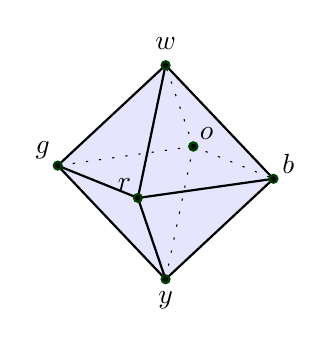
\begin{tikzpicture}%
  [x={(-0.860769cm, -0.121512cm)},
  y={(0.508996cm, -0.205391cm)},
  z={(-0.000053cm, 0.971107cm)},
  scale=1,
  back/.style={loosely dotted, thin},
  edge/.style={black, thick},
  facet/.style={fill=blue!95!black,fill opacity=0.1},
  vertex/.style={inner sep=1pt,circle,draw=green!25!black,fill=black,thick}]
\coordinate (-1, -1, 0) at (-1, -1, 0);
\coordinate (-1, 1, 0) at (-1, 1, 0);
\coordinate (0, 0, -1) at (0, 0, -1);
\coordinate (0, 0, 1) at (0, 0, 1);
\coordinate (1, -1, 0) at (1, -1, 0);
\coordinate (1, 1, 0) at (1, 1, 0);
%% Drawing edges in the back
%%
\draw[edge,back] (-1, -1, 0) -- (-1, 1, 0);
\draw[edge,back] (-1, -1, 0) -- (0, 0, -1.4);
\draw[edge,back] (-1, -1, 0) -- (0, 0, 1.4);
\draw[edge,back] (-1, -1, 0) -- (1, -1, 0);
%% Drawing vertices in the back
%%
\node[vertex] at (-1, -1, 0)     {};
%% Drawing the facets
%%
\fill[facet] (1, 1, 0) -- (0, 0, -1.4) -- (1, -1, 0) -- cycle {};
\fill[facet] (1, 1, 0) -- (0, 0, 1.4) -- (1, -1, 0) -- cycle {};
\fill[facet] (1, 1, 0) -- (-1, 1, 0) -- (0, 0, 1.4) -- cycle {};
\fill[facet] (1, 1, 0) -- (-1, 1, 0) -- (0, 0, -1.4) -- cycle {};
%% Drawing edges in the front
%%
\draw[edge] (-1, 1, 0) -- (0, 0, -1.4);
\draw[edge] (-1, 1, 0) -- (0, 0, 1.4);
\draw[edge] (-1, 1, 0) -- (1, 1, 0);
\draw[edge] (0, 0, -1.4) -- (1, -1, 0);
\draw[edge] (0, 0, -1.4) -- (1, 1, 0);
\draw[edge] (0, 0, 1.4) -- (1, -1, 0);
\draw[edge] (0, 0, 1.4) -- (1, 1, 0);
\draw[edge] (1, -1, 0) -- (1, 1, 0);
%% Drawing the vertices in the front
%%
\begin{scope}[nodes=vertex]
\node[label=above right:\( b \)] at (-1, 1, 0)     {};
\node[label=below:\( y \)] at (0, 0, -1.4)     {};
\node[label=above:\( w \)] at (0, 0, 1.4)     {};
\node[label=above left:\( g \)] at (1, -1, 0)     {};
\node[label=above left:\( r \)] at (1, 1, 0)     {};
\node[label=above right:\( o \)] at (-1, -1, 0)     {};
\end{scope}
\end{tikzpicture}
\caption{The HIT \( \oo \) which has 6 points, 12 1-paths, 8 2-paths.}
\end{figure}

\caption{The HIT \( \oo \) which has 6 points, 12 1-paths, 8 2-paths.}
\end{figure}

We have obvious maps \( \oo_0\xrightarrow[]{i_0} \oo_1\xrightarrow[]{i_1} \oo \) that include each skeleton into the next-higher-dimensional skeleton.

\subsubsection{\texorpdfstring{\( \link \), \( \xbox \), and \( \xdisk \)}{link, xbox, and xdisk}}

Here we'll define combinatorial versions of tangent spaces and tangent circles, in the special case where every vertex has four neighbors.

Combinatorial spaces have a concept called the \emph{link} of a vertex, which will be the main tool by which we connect with manifold theory. The vertices in the link are the vertices that are one edge away from the given point (its immediate neighbors), and the edges in the link are the edges connecting the neighbors to each other. If the link of an \( n \)-dimensional combinatorial space is always a combinatorial \( n-1 \)-sphere, then we say the space is a \emph{combinatorial triangulation}. We will look only at HITs that have a link that is merely equivalent to \( C_4 \). So first we need notation for a connected component of the universe:

\begin{mydef}
If we have \( X:\Type \) then we define \( \BAut X\defeq \sit{Y:\Type} ||X=Y||_{-1} \). 
\end{mydef}

Denote by \( abcd:\BAut C_4 \) the HIT with vertices \( a, b, c, d \) and edges \( ab, bc, cd, da \) which clearly has various isomorphisms with \( C_4 \).

We can now define a map \( \link:\oo_0\to\BAut C_4 \). Extending this later on to the 1-skeleton and 2-skeleton will take us into differential geometry!

\begin{mydef}
\( \link:\oo_0\to\BAut C_4 \) is given by induction:
\begin{align*}
\link(w) &= brgo \\
\link(y) &= bogr \\
\link(b) &= woyr \\
\link(r) &= wbyg \\
\link(g) &= wryo \\
\link(o) &= wgyb
\end{align*}
We chose these orderings for the vertices by standing at the given vertex and enumerating the link in clockwise order, starting from \( w \) if possible, else \( b \).
\end{mydef}

\begin{figure}[h]
\centering
\begin{figure}[h]
\centering
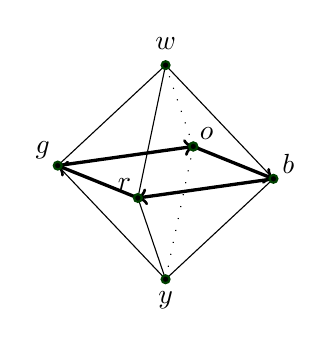
\begin{tikzpicture}%
  [x={(-0.860769cm, -0.121512cm)},
  y={(0.508996cm, -0.205391cm)},
  z={(-0.000053cm, 0.971107cm)},
  scale=1,
  eqback/.style={->, very thick},
  back/.style={loosely dotted, thin},
  eqedge/.style={->, very thick},
  edge/.style={black, thin},
  facet/.style={fill=blue!95!black,fill opacity=0.0},
  vertex/.style={inner sep=1pt,circle,draw=green!25!black,fill=black,thick}]
\coordinate (-1, -1, 0) at (-1, -1, 0);
\coordinate (-1, 1, 0) at (-1, 1, 0);
\coordinate (0, 0, -1) at (0, 0, -1);
\coordinate (0, 0, 1) at (0, 0, 1);
\coordinate (1, -1, 0) at (1, -1, 0);
\coordinate (1, 1, 0) at (1, 1, 0);
%% Drawing edges in the back
%%
\draw[edge,eqback] (-1, -1, 0) -- (-1, 1, 0);
\draw[edge,back] (-1, -1, 0) -- (0, 0, -1.4);
\draw[edge,back] (-1, -1, 0) -- (0, 0, 1.4);
\draw[edge,eqback] (1, -1, 0) -- (-1, -1, 0);
%% Drawing vertices in the back
%%
\node[vertex] at (-1, -1, 0)     {};
%% Drawing the facets
%%
\fill[facet] (1, 1, 0) -- (0, 0, -1.4) -- (1, -1, 0) -- cycle {};
\fill[facet] (1, 1, 0) -- (0, 0, 1.4) -- (1, -1, 0) -- cycle {};
\fill[facet] (1, 1, 0) -- (-1, 1, 0) -- (0, 0, 1.4) -- cycle {};
\fill[facet] (1, 1, 0) -- (-1, 1, 0) -- (0, 0, -1.4) -- cycle {};
%% Drawing edges in the front
%%
\draw[edge] (-1, 1, 0) -- (0, 0, -1.4);
\draw[edge] (-1, 1, 0) -- (0, 0, 1.4);
\draw[eqedge] (-1, 1, 0) -- (1, 1, 0);
\draw[edge] (0, 0, -1.4) -- (1, -1, 0);
\draw[edge] (0, 0, -1.4) -- (1, 1, 0);
\draw[edge] (0, 0, 1.4) -- (1, -1, 0);
\draw[edge] (0, 0, 1.4) -- (1, 1, 0);
\draw[eqedge] (1, 1, 0) -- (1, -1, 0);
%% Drawing the vertices in the front
%%
\begin{scope}[nodes=vertex]
\node[label=above right:\( b \)] at (-1, 1, 0)     {};
\node[label=below:\( y \)] at (0, 0, -1.4)     {};
\node[label=above:\( w \)] at (0, 0, 1.4)     {};
\node[label=above left:\( g \)] at (1, -1, 0)     {};
\node[label=above left:\( r \)] at (1, 1, 0)     {};
\node[label=above right:\( o \)] at (-1, -1, 0)     {};
\end{scope}
\end{tikzpicture}

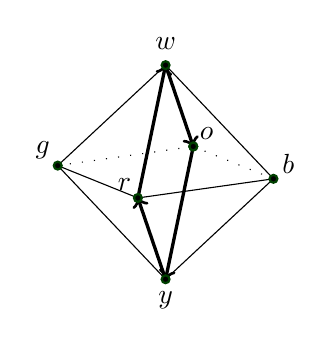
\begin{tikzpicture}%
  [x={(-0.860769cm, -0.121512cm)},
  y={(0.508996cm, -0.205391cm)},
  z={(-0.000053cm, 0.971107cm)},
  scale=1,
  eqback/.style={->, very thick},
  back/.style={loosely dotted, thin},
  eqedge/.style={->, very thick},
  edge/.style={black, thin},
  facet/.style={fill=blue!95!black,fill opacity=0.0},
  vertex/.style={inner sep=1pt,circle,draw=green!25!black,fill=black,thick}]
\coordinate (-1, -1, 0) at (-1, -1, 0);
\coordinate (-1, 1, 0) at (-1, 1, 0);
\coordinate (0, 0, -1) at (0, 0, -1);
\coordinate (0, 0, 1) at (0, 0, 1);
\coordinate (1, -1, 0) at (1, -1, 0);
\coordinate (1, 1, 0) at (1, 1, 0);
%% Drawing edges in the back
%%
\draw[edge,back] (-1, -1, 0) -- (-1, 1, 0);
\draw[edge,eqback] (-1, -1, 0) -- (0, 0, -1.4);
\draw[edge,eqback] (0, 0, 1.4) -- (-1, -1, 0);
\draw[edge,back] (1, -1, 0) -- (-1, -1, 0);
%% Drawing vertices in the back
%%
\node[vertex] at (-1, -1, 0)     {};
%% Drawing the facets
%%
\fill[facet] (1, 1, 0) -- (0, 0, -1.4) -- (1, -1, 0) -- cycle {};
\fill[facet] (1, 1, 0) -- (0, 0, 1.4) -- (1, -1, 0) -- cycle {};
\fill[facet] (1, 1, 0) -- (-1, 1, 0) -- (0, 0, 1.4) -- cycle {};
\fill[facet] (1, 1, 0) -- (-1, 1, 0) -- (0, 0, -1.4) -- cycle {};
%% Drawing edges in the front
%%
\draw[edge] (-1, 1, 0) -- (0, 0, -1.4);
\draw[edge] (-1, 1, 0) -- (0, 0, 1.4);
\draw[edge] (-1, 1, 0) -- (1, 1, 0);
\draw[edge] (0, 0, -1.4) -- (1, -1, 0);
\draw[eqedge] (0, 0, -1.4) -- (1, 1, 0);
\draw[edge] (0, 0, 1.4) -- (1, -1, 0);
\draw[eqedge] (1, 1, 0) -- (0, 0, 1.4) ;
\draw[edge] (1, 1, 0) -- (1, -1, 0);
%% Drawing the vertices in the front
%%
\begin{scope}[nodes=vertex]
\node[label=above right:\( b \)] at (-1, 1, 0)     {};
\node[label=below:\( y \)] at (0, 0, -1.4)     {};
\node[label=above:\( w \)] at (0, 0, 1.4)     {};
\node[label=above left:\( g \)] at (1, -1, 0)     {};
\node[label=above left:\( r \)] at (1, 1, 0)     {};
\node[label=above right:\( o \)] at (-1, -1, 0)     {};
\end{scope}
\end{tikzpicture}

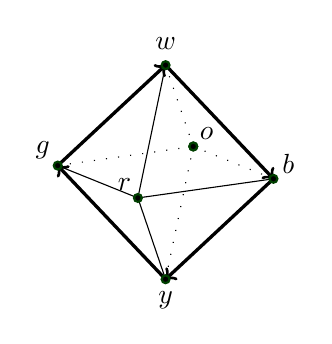
\begin{tikzpicture}%
  [x={(-0.860769cm, -0.121512cm)},
  y={(0.508996cm, -0.205391cm)},
  z={(-0.000053cm, 0.971107cm)},
  scale=1,
  eqback/.style={->, very thick},
  back/.style={loosely dotted, thin},
  eqedge/.style={->, very thick},
  edge/.style={black, thin},
  facet/.style={fill=blue!95!black,fill opacity=0.0},
  vertex/.style={inner sep=1pt,circle,draw=green!25!black,fill=black,thick}]
\coordinate (-1, -1, 0) at (-1, -1, 0);
\coordinate (-1, 1, 0) at (-1, 1, 0);
\coordinate (0, 0, -1) at (0, 0, -1);
\coordinate (0, 0, 1) at (0, 0, 1);
\coordinate (1, -1, 0) at (1, -1, 0);
\coordinate (1, 1, 0) at (1, 1, 0);
%% Drawing edges in the back
%%
\draw[edge,back] (-1, -1, 0) -- (-1, 1, 0);
\draw[edge,back] (-1, -1, 0) -- (0, 0, -1.4);
\draw[edge,back] (-1, -1, 0) -- (0, 0, 1.4);
\draw[edge,back] (1, -1, 0) -- (-1, -1, 0);
%% Drawing vertices in the back
%%
\node[vertex] at (-1, -1, 0)     {};
%% Drawing the facets
%%
\fill[facet] (1, 1, 0) -- (0, 0, -1.4) -- (1, -1, 0) -- cycle {};
\fill[facet] (1, 1, 0) -- (0, 0, 1.4) -- (1, -1, 0) -- cycle {};
\fill[facet] (1, 1, 0) -- (-1, 1, 0) -- (0, 0, 1.4) -- cycle {};
\fill[facet] (1, 1, 0) -- (-1, 1, 0) -- (0, 0, -1.4) -- cycle {};
%% Drawing edges in the front
%%
\draw[eqedge] (-1, 1, 0) -- (0, 0, -1.4);
\draw[eqedge] (0, 0, 1.4) -- (-1, 1, 0);
\draw[edge] (-1, 1, 0) -- (1, 1, 0);
\draw[eqedge] (0, 0, -1.4) -- (1, -1, 0);
\draw[edge] (0, 0, -1.4) -- (1, 1, 0);
\draw[eqedge] (1, -1, 0) -- (0, 0, 1.4);
\draw[edge] (0, 0, 1.4) -- (1, 1, 0);
\draw[edge] (1, 1, 0) -- (1, -1, 0);
%% Drawing the vertices in the front
%%
\begin{scope}[nodes=vertex]
\node[label=above right:\( b \)] at (-1, 1, 0)     {};
\node[label=below:\( y \)] at (0, 0, -1.4)     {};
\node[label=above:\( w \)] at (0, 0, 1.4)     {};
\node[label=above left:\( g \)] at (1, -1, 0)     {};
\node[label=above left:\( r \)] at (1, 1, 0)     {};
\node[label=above right:\( o \)] at (-1, -1, 0)     {};
\end{scope}
\end{tikzpicture}
\caption{The equators for \( w, b, r \).}
\end{figure}
\caption{\( \link \) for the verticies \( w, b\) and \( r \).}
\label{fig:triangle_of_equators}
\end{figure}

Besides the link we also want to consider the 5-pointed object that includes the vertex itself and the edges connecting it to the vertices in the link. We will call such a shape an \emph{xbox} since it is a square with both diagonals. We will denote xboxes by extending the square notation with a fifth letter to indicate the center of the xbox. For example, we can define an xbox \( C_{4c} \) as follows:

\begin{mydef}
The higher inductive type \( C_{4c} \) with center \( c \), also denoted \( c_1c_2c_3c_4c \).
\begin{align*}
C_{4c} &: \Type \\
c_1, c_2, c_3, c_4, c &: C_{4c} \\
c_1c_2 &: c_1 = c_2 \\
c_2c_3 &: c_2 = c_3 \\
c_3c_4 &: c_3 = c_4 \\
c_4c_1 &: c_4 = c_1 \\
c_1c &: c_1 = c \\
c_2c &: c_2 = c \\
c_3c &: c_3 = c \\
c_4c &: c_4 = c 
\end{align*}
\end{mydef}

And we get a map \( \xbox:\oo_0\to\Type \) similarly to \( \link \).
\begin{mydef}
\( \xbox:\oo_0\to\BAut C_{4c} \) is given by induction:
\begin{align*}
\xbox(w) &= brgow \\
\xbox(y) &= bogry \\
\xbox(b) &= woyrb \\
\xbox(r) &= wbygr \\
\xbox(g) &= wryog \\
\xbox(o) &= wgybo
\end{align*}
\end{mydef}

Finally we want to consider the 2-type that fills in the faces of the xbox. This is a contractible type we will call an \emph{xdisk}. 

\begin{mydef}
The higher inductive type \( C_{4c\xdisk} \) with center \( c \), also denoted \( c_1c_2c_3c_4c_\xdisk \).
\begin{align*}
C_{4c\xdisk} &: \Type \\
c_1, c_2, c_3, c_4, c &: C_{4c\xdisk} \\
c_1c_2 &: c_1 = c_2 \\
c_2c_3 &: c_2 = c_3 \\
c_3c_4 &: c_3 = c_4 \\
c_4c_1 &: c_4 = c_1 \\
c_1c &: c_1 = c \\
c_2c &: c_2 = c \\
c_3c &: c_3 = c \\
c_4c &: c_4 = c \\
c_1c_2c &: c_1c_2\cdot c_2c\cdot c_1c^{-1} = \refl \\
c_2c_3c &: c_2c_2\cdot c_3c\cdot c_2c^{-1} = \refl \\
c_3c_4c &: c_3c_2\cdot c_4c\cdot c_3c^{-1} = \refl \\
c_4c_1c &: c_4c_2\cdot c_1c\cdot c_4c^{-1} = \refl
\end{align*}
\end{mydef}

We can define \( \xdisk:\oo_0\to\BAut C_{4c\xdisk} \) by filling in the triangles in \( \xbox \).

\begin{mydef}
\( \xdisk:\oo_0\to\BAut C_{4c\xdisk} \) is given by induction:
\begin{align*}
\xbox(w) &= brgow_\xdisk \\
\xbox(y) &= bogry_\xdisk \\
\xbox(b) &= woyrb_\xdisk \\
\xbox(r) &= wbygr_\xdisk \\
\xbox(g) &= wryog_\xdisk \\
\xbox(o) &= wgybo_\xdisk
\end{align*}
\end{mydef}

\subsubsection{Extending \texorpdfstring{\( \link \)}{link}}

Note that \( \BAut C_4 \) is of homotopy dimension at least 2, just as \( \oo \) is. The paths are isomorphisms between types that are merely equivalent to squares, and the 2-paths are homotopies between these. We can make further use of Figure~\ref{fig:triangle_of_equators} by imagining how \( \link \) changes as we slide from point to point. Sliding from \( w \) to \( b \) and tipping the link as we go, we see \( r\mapsto r \) and \( o\mapsto o \) because those lie on the axis of rotation. Then \( g\mapsto w \) and \( b\mapsto y \). 

The full map on the 1-skeleton is:
\begin{mydef}
Define \( T_1:\oo\to\BAut C_4 \) on just the 1-skeleton by extending \( \link \) as follows:
Transport away from \( w \):
\begin{itemize}
\item \( T_1(wb):[b, r, g, o]\mapsto [y, r, w, o] \) (\( r, o \) fixed)
\item \( T_1(wr):[b, r, g, o]\mapsto [b, y, g, w] \) (\( b, g \) fixed)
\item \( T_1(wg):[b, r, g, o]\mapsto [w, r, y, o] \)
\item \( T_1(wo):[b, r, g, o]\mapsto [b, w, g, y] \)
\end{itemize}
Transport away from \( y \):
\begin{itemize}
\item \( T_1(yb):[b, o, g, r]\mapsto [w, o, y, r] \)
\item \( T_1(yr):[b, o, g, r]\mapsto [b, y, g, w] \)
\item \( T_1(yg):[b, o, g, r]\mapsto [y, o, w, r] \)
\item \( T_1(yo):[b, o, g, r]\mapsto [b, w, g, y] \)
\end{itemize}
Transport along the equator:
\begin{itemize}
\item \( T_1(br):[w, o, y, r]\mapsto [w, b, y, g] \) 
\item \( T_1(rg):[w, b, y, g]\mapsto [w, r, y, o] \)
\item \( T_1(go):[w, r, y, o]\mapsto [w, g, y, b] \)
\item \( T_1(ob):[w, g, y, b]\mapsto [w, o, y, r] \)
\end{itemize}
\end{mydef}

It's very important to be able to visualize what \( T_1 \) does to triangular paths such as \( wb\cdot br\cdot rw \) (which circulates around the boundary of face \( wbr \)). You can see it if you imagine Figure~\ref{fig:triangle_of_equators} as the frames of a short movie. Or you can place your palm over the top of a cube and note where your fingers are pointing, then slide your hand to an equatorial face, then along the equator, then back to the top. The answer is: you come back rotated clockwise by a quarter-turn. 

\begin{mydef}
The map \( R:C_4\to C_4 \) rotates by one quarter turn, one ``click":
\begin{itemize}
\item \( R(c_1) = c_2 \)
\item \( R(c_2) = c_3 \)
\item \( R(c_3) = c_4 \)
\item \( R(c_4) = c_1 \)
\item \( R(c_1c_2) = c_2c_3 \)
\item \( R(c_2c_3) = c_3c_4 \)
\item \( R(c_3c_4) = c_4c_1 \)
\item \( R(c_4c_1) = c_1c_2 \)
\end{itemize}
\end{mydef}

Now let's extend \( T_1 \) to all of \( \oo \) by providing values for the eight faces. The face \( wbr \) is a path from \( \refl_w \) to the concatenation \( wb\cdot br\cdot rw \), and so the image of \( wbr \) under the extended version of \( T_1 \) must be a homotopy from \( \refl_{T_1(w)} \) to \( T_1(wb\cdot br\cdot rw) \).

\begin{mydef}
Define \( T_2:\oo\to\BAut C_4 \) by extending \( T_1 \) to the faces as follows:
\begin{itemize}
\item \( T_2(wbr)=H_R \) 
\item \( T_2(wrg)=H_R \)
\item \( T_2(wgo)=H_R \)
\item \( T_2(ybo)=H_R \)
\item \( T_2(yrb)=H_R \) 
\item \( T_2(ygr)=H_R \)
\item \( T_2(yog)=H_R \)
\item \( T_2(ybo)=H_R \)
\end{itemize}
where \( H_R:R=\refl \) is the obvious homotopy.
\end{mydef}

All the faces do the same thing: they map to a homotopy between the identity and clockwise rotation by a quarter turn. Concatenating the eight faces in the 2-groupoid \( \oo \) would then map to a homotopy between the identity and two full rotations. This makes visible in HoTT the link between curvature and the euler characteristic (which is 2 for the octahedron).

\subsection{The torus}

We can define a combinatorial torus as a similar HIT. Each vertex will again have four neighbors and all the links will be merely equal to \( C_4 \). See Figure~\ref{fig:torus}. Hmm that one isn't a combinatorial manifold so never mind!

In this case it should be intuitively obvious that transport around the boundary of any face is the identity, corresponding to the torus being flat.

\begin{figure}[h]
\centering
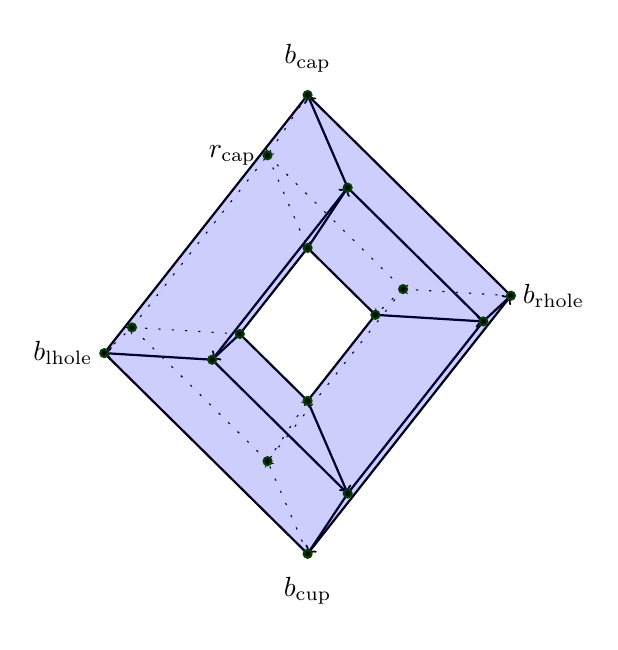
\begin{tikzpicture}%
  [x={(-0.860769cm, -0.121512cm)},
  y={(0.508996cm, -0.205391cm)},
  z={(-0.000053cm, 0.971107cm)},
  scale=1,
  back/.style={loosely dotted, thin},
  edge/.style={->,black, thick},
  line/.style={black, thick},
  facet/.style={fill=blue!95!black,fill opacity=0.1},
  vertex/.style={inner sep=1pt,circle,draw=green!25!black,fill=black,thick}]
\coordinate (r_cap) at (0, -1, 5);
\coordinate (g_cap) at (0, 0, 4 );
\coordinate (o_cap) at (0, 1, 5 );
\coordinate (b_cap) at (0, 0, 6 );

\coordinate (r_cup) at (0, -1, 1);
\coordinate (g_cup) at (0, 0, 2 );
\coordinate (o_cup) at (0, 1, 1 );
\coordinate (b_cup) at (0, 0, 0 );

\coordinate (r_ohole) at (-2, -1, 3);
\coordinate (g_ohole) at (-1, 0,  3);
\coordinate (o_ohole) at (-2, 1,  3);
\coordinate (b_ohole) at (-3, 0,  3);

\coordinate (r_rhole) at (2, -1, 3);
\coordinate (g_rhole) at (1, 0,  3);
\coordinate (o_rhole) at (2, 1,  3);
\coordinate (b_rhole) at (3, 0,  3);

\draw[edge,back] (r_cap) -- (g_cap);
\draw[edge]      (g_cap) -- (o_cap);
\draw[edge]      (o_cap) -- (b_cap);
\draw[edge,back] (b_cap) -- (r_cap);

\draw[edge,back] (r_cup) -- (g_cup);
\draw[edge]      (g_cup) -- (o_cup);
\draw[edge]      (o_cup) -- (b_cup);
\draw[edge,back] (b_cup) -- (r_cup);

\draw[edge,back] (r_ohole) -- (g_ohole);
\draw[edge]      (g_ohole) -- (o_ohole);
\draw[edge]      (o_ohole) -- (b_ohole);
\draw[edge,back] (b_ohole) -- (r_ohole);

\draw[edge,back] (r_rhole) -- (g_rhole);
\draw[edge]      (g_rhole) -- (o_rhole);
\draw[edge]      (o_rhole) -- (b_rhole);
\draw[edge,back] (b_rhole) -- (r_rhole);

\draw[line,back] (r_cap) --   (r_ohole);
\draw[line,back] (r_ohole) -- (r_cup);
\draw[line,back] (r_cup) --   (r_rhole);
\draw[line,back] (r_rhole) -- (r_cap);

\draw[line] (g_cap) --   (g_ohole);
\draw[line] (g_ohole) -- (g_cup);
\draw[line] (g_cup) --   (g_rhole);
\draw[line] (g_rhole) -- (g_cap);

\draw[line] (o_cap) --   (o_ohole);
\draw[line] (o_ohole) -- (o_cup);
\draw[line] (o_cup) --   (o_rhole);
\draw[line] (o_rhole) -- (o_cap);

\draw[line] (b_cap) --   (b_ohole);
\draw[line] (b_ohole) -- (b_cup);
\draw[line] (b_cup) --   (b_rhole);
\draw[line] (b_rhole) -- (b_cap);

\fill[facet] (r_cap) -- (r_ohole) -- (g_ohole) -- (g_cap) -- cycle {};
\fill[facet] (r_cap) -- (r_rhole) -- (g_rhole) -- (g_cap) -- cycle {};
\fill[facet] (r_cap) -- (r_ohole) -- (b_ohole) -- (b_cap) -- cycle {};
\fill[facet] (r_cap) -- (r_rhole) -- (b_rhole) -- (b_cap) -- cycle {};

\fill[facet] (o_cap) -- (o_ohole) -- (g_ohole) -- (g_cap) -- cycle {};
\fill[facet] (o_cap) -- (o_rhole) -- (g_rhole) -- (g_cap) -- cycle {};
\fill[facet] (o_cap) -- (o_ohole) -- (b_ohole) -- (b_cap) -- cycle {};
\fill[facet] (o_cap) -- (o_rhole) -- (b_rhole) -- (b_cap) -- cycle {};

\fill[facet] (r_cup) -- (r_ohole) -- (g_ohole) -- (g_cup) -- cycle {};
\fill[facet] (r_cup) -- (r_rhole) -- (g_rhole) -- (g_cup) -- cycle {};
\fill[facet] (r_cup) -- (r_ohole) -- (b_ohole) -- (b_cup) -- cycle {};
\fill[facet] (r_cup) -- (r_rhole) -- (b_rhole) -- (b_cup) -- cycle {};

\fill[facet] (o_cup) -- (o_ohole) -- (g_ohole) -- (g_cup) -- cycle {};
\fill[facet] (o_cup) -- (o_rhole) -- (g_rhole) -- (g_cup) -- cycle {};
\fill[facet] (o_cup) -- (o_ohole) -- (b_ohole) -- (b_cup) -- cycle {};
\fill[facet] (o_cup) -- (o_rhole) -- (b_rhole) -- (b_cup) -- cycle {};

\begin{scope}[nodes=vertex]
\node[label=left:\( r_{\mathrm{cap}} \)] at (r_cap) {};
\node at (g_cap) {};
\node at (o_cap) {};
\node[label=above:\( b_{\mathrm{cap}} \)] at (b_cap) {};
\node at (r_cup) {};
\node at (g_cup) {};
\node at (o_cup) {};
\node[label=below:\( b_{\mathrm{cup}} \)] at (b_cup) {};
\node at (r_ohole) {};
\node at (g_ohole) {};
\node at (o_ohole) {};
\node[label=right:\( b_{\mathrm{rhole}} \)] at (b_ohole) {};
\node at (r_rhole) {};
\node at (g_rhole) {};
\node at (o_rhole) {};
\node[label=left:\( b_{\mathrm{lhole}} \)] at (b_rhole) {};
\end{scope}
\end{tikzpicture}

\caption{Torus. The squares are nicknamed cap, cup, lhole, and rhole. Each one has a \( b, r, g, o \) vertex, in that order when following the arrows. All the \( b \)s are on the outer corners, all the \( r \)s are in the back, and so on.}
\label{fig:torus}
\end{figure}

\subsection{Combinatorial manifolds}

(This section is not quite off the ground.)

The combinatorial structure we have in mind is a nerve of a good open cover. What do we know about which smooth manifolds have such covers? While we're at it, let's survey all the combinatorial-flavored spaces and survey what smooth manifolds are homotopy equivalent to which structures.

What topological manifolds are equivalent to a CW complex? The answer is the composition of a few results summarized by Allen Hatcher\footnote{\url{https://mathoverflow.net/questions/201944/topological-n-manifolds-have-the-homotopy-type-of-n-dimensional-cw-complexes}} (citing \cite{kirby_siebenmann} and \cite{freedman_quinn}):

\begin{quote}
Every topological manifold has a handlebody structure except in dimension 4, where a 4-manifold has a handlebody structure if and only if it is smoothable. This is a theorem on page 136 of Freedman and Quinn's book ``Topology of 4-Manifolds'', with a reference given to the Kirby-Siebenmann book for the higher-dimensional case. It is then an elementary fact that an \( n \)-manifold with a handlebody structure is homotopy equivalent to a CW complex with one \( k \)-cell for each \( k \)-handle, so in particular there are no cells of dimension greater than \( n \). At least in the compact case a manifold with a handlebody structure is in fact homeomorphic to a CW complex with \( k \)-cells corresponding to \( k \)-handles; see page 107 of Kirby-Siebenmann. This probably holds in the noncompact case as well, though I don't know a reference.
\end{quote}


